% !TEX root = ../main.tex
\chapter{引言}
\label{cha:intro}

\section{选题背景}
\label{sec:background}
自人类文明起源至今,交通便扮演着促进贸易往来,加强文化交流的重要角色,尤其是随着现代社会交通工具,基础设施的迅猛发展,人类的活动范围极大扩张,流动成本极大减小,人们的交流交通的需求也随之增大。在这样的背景下,道路通行能力的限制已经成为制约人们通行需求的重要因素。以北京市为例,截止2014 年末,全市机动车保有量559.1 万辆,其中私人汽车保有量达到437.2 万辆,私人轿车保有量316.5 万辆。以$\SI{4}{m}$来估计单辆车长,那么全长约$\SI{146}{km}$的北京二环、三环和四环3 条快速路全排满也最多只能容纳约32 万辆,不足全市机动车的5\%。有限的通行能力与巨大的私家车保有量之间形成了剧烈的矛盾,导致北京的交通状况不容乐观。除通行能力之外,对于减少排放、提高安全性的需求也日益上升\cite{Ploeg2014Analysis}。图\ref{fig:traffic}(来源:国家统计局 \url{http://data.stats.gov.cn/easyquery.htm?cn=C01&zb=A0S0D01&sj=2015})显示了我国交通安全现状。从图中可以看出,虽然我国交通安全正在逐渐改善,但仍有很大的提高空间。

\begin{figure}[htbp]
\begin{minipage}[t]{0.4\linewidth}
\centering
\begin{tikzpicture}[x=0.1cm, font=\sffamily]
\begin{axis}[
xlabel={年份},
ylabel={交通事故发生数总计(起)},
grid=major,
ymin=0,
grid style={dashed,gray!30},
scale only axis,
width=\textwidth,
/pgf/number format/.cd, 1000 sep={},
% x unit=\si{\volt},
% y unit=\si{\ampere},
% legend pos=south east,
% legend entries={Concrete,Linoleum},
]
\addplot table [x=year,y=per] {stat/traffic_accident.dat};
\end{axis}
\end{tikzpicture}
\end{minipage}%
\hspace{+2cm}
\begin{minipage}[t]{0.4\linewidth}
\centering
\begin{tikzpicture}[font=\sffamily]
\begin{axis}[
xlabel={年份},
ylabel={交通事故死亡人数总计(人)},
grid=major,
grid style={dashed,gray!30},
ymin=0,
scale only axis,
width=\textwidth,
/pgf/number format/.cd, 1000 sep={},
% x unit=\si{\volt},
% y unit=\si{\ampere},
% legend pos=south east,
% legend entries={Concrete,Linoleum},
]
\addplot table [x=year,y=per] {stat/traffic_dead.dat};
\end{axis}
\end{tikzpicture}
\end{minipage}
\captionsetup{margin=3.cm}
\caption[交通事故统计图]{2006-2015年全国道路交通事故总数(左)与交通事故死亡人数(右)统计图}
\label{fig:traffic}
\end{figure}

新一代智能车技术的发展为解决交通问题提供了新途径。智能车(英文文献中常称为 Connected Automated Vehicle,简记作 CAV)又可以分为智能网联车(Connected vehicle)和自动驾驶车(Autonomous vehicle),但这两类车的技术又可以进行结合,如图\ref{fig:IV}(来源:\url{http://slideplayer.com/slide/4589633/})。\textbf{网联车} 是指搭载先进的车载传感器、控制器、执行器等装置,并融合现代通信与网络技术,实现车与X(车、路、人、后台等)的信息交换,具备复杂的环境感知、智能决策、协同控制和执行等功能,可实现安全、舒适、节能、高效行驶。\textbf{自动驾驶汽车}(也称无人驾驶汽车、自驾车、机器人汽车\cite{Thrun2010Toward},以下简称\textbf{无人车})是一种无需人工输入,能够感知周围环境并自主导航的车辆。无人车系统融合了许多技术,例如使用视频摄像头、激光测距仪、雷达传感器等来感知周围环境,使用GPS技术获取道路信息,运用计算机视觉方法处理获得的信息。无人车技术在业界广受关注,例如谷歌\cite{google2017self}、特斯拉\cite{tesla2017model}等公司都已经推出了无人车产品。但是截止2017年2月,世界范围内获准上路的无人车中还没能实现完全自主。

\begin{figure}
\centering
\href{http://slideplayer.com/slide/4589633/}{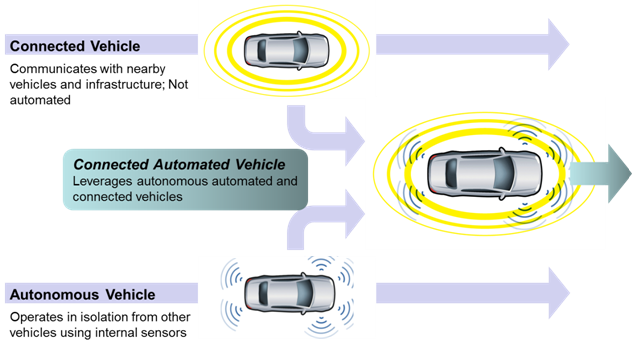
\includegraphics[width=13cm]{IV.png}}
\caption{网联车与自动驾驶车}
\label{fig:IV}
\end{figure}

将车路协同技术和无人驾驶技术融合,是智能车发展的必然趋势。新一代智能车不仅可以通过感知技术提高对驾驶环境的认知能力,还将通过网联技术实现信息交互,提升车辆运行效率、降低车辆能耗提升交通系统性等方面有极大的潜力。基于这样的平台,对于智能车的决策方案有望从单决策传统智能车决策方法,走向对多智车以群体行为效果为主的决策方案的研究,从而进一步提高系统整体的运行效率和安全性。

对于这样复杂系统的研究和群决策机理的分析,可以从相对简单的场景开始,再进一步向复杂场景进行推广。因此,本课题将以完全可控的智能车(CAV)为研究对象,基于车路协同平台,研究多智能车系统在车辆交汇口的群决策问题。

\section{研究现状}
本章对于同本课题相关的研究进行文献综述。具体地,\ref{sec:VIC}节总结了世界范围内车路协同基础设施的最新进展,为多智能车的群决策提供支持;\ref{sec:self}节总结了无人车的发展历史和基本概念;\ref{sec:single}节对智能车的运动学模型和决策问题进行了概述;\ref{ssec:intro:summary}节对研究现状进行了总结。

\subsection{车路协同系统的发展}
\label{sec:VIC}
车路协同通过部署新型基础设施,实现车车交互、车路交互,以提高交通系统的安全性和运行效率。近几年来,无人车技术,通信技术,GPS定位技术,以及云计算等新技术的发展在智能交通领域的应用,进一步推动了车路协同技术的应用与升级。

\begin{enumerate}[wide=\parindent]
\item \textbf{国外车路协同研究现状}
\begin{enumerate}[wide=\parindent,label=(\arabic*)]
\item 美国  IntelliDrive。 美国车路协同系统(vehicle infrastructure integration, VII),后更名为 IntelliDrive,是由美国联邦公路局 (FHWA)、AASHTO、各州交通部 (State DOT)、汽车产业联盟、ITS American 等机构联合参与,着眼于安全性、交通机动性和环境友好性。项目在未来还将整合主动安全、电子支付等先进技术,进一步提高道路通行的效率和安全性。

\item 日本  SmartWay。 日本的车路协同系统 Smartway \cite{Hiroshi2005Smartway} 由23家企业与政府共同发起,其发展重点在整合日本各项 ITS的功能,促进基础道路设施改善、提高交通运输效率、并促进智能车(在此处是指 advanced safety vehicle, ASV)\cite{Chapman2010USING}的研发。该项目已经在东京区、三大都会区进行了试验,同时还能提供辅助驾驶、图像采集、停车场电子付费等服务。

\item 欧洲  eSafty。 该计划2003年9月得到欧盟委员会的认可并列入欧盟计划,旨在利用最新信息与通信技术,
加快研发并集成安全系统,为道路交通提供全面安全解决方案。欧洲自2010年,对智能车展开了实地测试。
\end{enumerate}

\item \textbf{国内车路协同系统研究现状}

我国在车路协同方面的研究起步较晚。近年来,高校与科研单位逐步开展了车路协同技术的研究\cite{Tian2010A,Danno2009VEHICLE}。2010 年,国家“十二五” 高技术研究发展研究计划所支持的“智能车路协同关键技术研究”主题项目,是我国第一个国家级的车路协同项目。该项目由清华大学牵头,研究团队囊括了国内顶尖的科研院所和汽车制造企业,实力强劲。项目中,研究团队针对车车交互、车路交互、协同控制与大规模仿真等关键技术开展研究工作,获得了丰硕成果。在清华河北研究院廊坊实验场,建设了一条包含两个十字路口和一条1.3km实验路段的测试环境,用于车路协同应用和交互试验,取得了一系列成果。项目组还提出了基于车路协同技术我国新一代ITS 体系框架,突出了车路协同系统的核心地位,使得所有ITS 服务子系统均依托于车路协同系统的平台建立,形成一个高效的有机整体。
\end{enumerate}

\subsection{无人车}
\label{sec:self}

无人车即前文所述的自动驾驶车。本节总结了无人车控制技术发展的历史,和无人车的自动程度分级,为后文具体综述无人车决策控制算法提供了背景知识。

\begin{enumerate}[wide=\parindent]
\item \textbf{无人车发展历程}

无人车技术具有悠久的历史。早在20世纪20年代,无人车的构想就已经出现\cite{Adrienne2016Your}。从20世纪80年代开始,关于无人车控制的理论研究陆续开始\cite{Dickmanns1988Dynamic}。1994年,作为 PROMETHEUS 工程\cite{eureka2016}的一部分,一辆名为 VaMP的无人车\cite{vamp2017}行驶了$1600$公里,其中$95\%$的路程是自动驾驶完成的。到2004年,为推动无人车技术的发展,第一次 DARPA 挑战在美国举办。挑战要求无人车自主完成长达150英里的越野赛道,与之前的无人车展示不同的是,比赛期间是不允许人工干预的。在此之后,又有许多关于无人车的比赛产生,值得一提的是在我国举办的 Intelligent Vehicle Future Challenges (IVFC)\cite{Xin2014China}。

\item \textbf{无人车自动程度等级}

SAE J3016 标准\cite{SO2014Taxonomy}将车辆自动化程度分为以下五个等级。
\begin{enumerate}[label=(\arabic*),wide=\parindent]
\item 等级0:车辆完全由人控制;

\item 等级1:包含基本驾驶辅助系统的车辆,例如自适应巡航控制系统,防抱死系统,电子稳定性控制\cite{Rajamani2011Vehicle}等;

\item 等级2:包含高级辅助系统的车辆,例如危害最小化纵/横向控制系统\cite{Gerdes2001A},紧急制动系统\cite{Brannstrom2010Model,Vahidi2003Research}等;

\item 等级3:车辆带有环境感知系统,能够在特定环境下全自动行驶,但在环境超出驾驶系统决策范围时仍需要人工干预,驾驶系统会让驾驶员接管并留出足够宽裕的转换时间;

\item 等级4:车辆能够在特定环境中全自动行驶,并且当驾驶员没有响应接管请求时,仍能安全控制车辆;

\item 等级5:在所有环境中都能够自动驾驶,不需要人为干预。
\end{enumerate}


\end{enumerate}

\subsection{智能车的决策问题}
\label{sec:single}
本节讨论关于智能车决策控制的具体算法,前三部分涉及单智能车的决策控制方法,第四部分讨论多智能车的决策控制,即群决策的相关问题。

\begin{enumerate}[wide=\parindent]
\item \textbf{无人车决策层次}
\label{sec:hierarchy}

无人车的控制系统,本质上是一个自动决策系统,该系统能够从传感器获取信息流,并结合对道路拓扑、交通规则、车辆运动学、传感器模型的先验知识,决定能够控制汽车运动的输出量。研究者普遍将无人车的决策问题分解为不同的层次,解决每个层面的控制问题。该问题可以分解为以下四层:路径规划层、行为决策层、动作决策层和车辆控制层\cite{paden2016survey},如图\ref{fig:decision0}。

\begin{figure}[htbp]
\centering
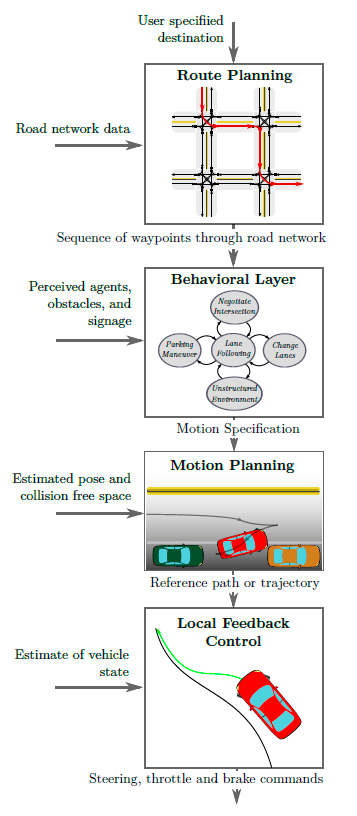
\includegraphics[width=9cm]{decision.png}
\caption{无人车决策层次\cite{paden2016survey}}
\label{fig:decision0}
\end{figure}
\begin{enumerate}[label=(\arabic*), wide=\parindent]
\item 路径规划层。这是无人车决策的最上层问题。通过将道路表示为有向网络,路径规划问题本质上就变成了一个最小费用流问题,可以采用 Dijkstra算法\cite{Dijkstra1959A},$A^*$启发式搜索\cite{Nilsson1969A}等。在路径规划的研究领域,目前已经出现了一系列算法,能够在经过一次预处理过后,在大陆规模的路网中以微秒量级输出最佳路径\cite{Goldberg2003Computing,Geisberger2012Exact}。

\item 行为决策层。当路径规划层求得了最佳路径之后,无人车需要根据路径进行导航,并和其他道路对象(人、车、障碍物等)进行交互。具体来说,输入一系列的路段,行为决策层需要根据感知到的路况信息(其他对象位置、信号灯等)决定驾驶行为(左转、右转、加速、减速、停车等)。由于周围环境和驾驶行为都可以被建模为有限集,可以使用有限状态机建模行为决策问题。其中状态为驾驶行为,状态转移由观察到的环境信息决定。

转移规则的学习可以使用传统的基于规则或基于统计的学习方法。在前述的 DARPA挑战赛中,大多数队伍都使用了基于规则的学习方法\cite{Buehler2009The}。近年来,由于人工智能的发展,业界也纷纷开始尝试使用深度学习、增强学习的方法,例如英伟达公司使用增强学习进行端到端无人车控制的工作\cite{Bojarski2016End}。

\item 轨迹规划层。当驾驶行为被确定后,选定的驾驶行为需要由轨迹规划层转化为特定的轨迹,提供给底层反馈控制单元沿轨迹运行。对于该路径可能存在障碍、曲率等一系列约束,优化的目标函数可能包括路径长度、人的舒适程度等。轨迹规划问题的精确解一般难以得到,在实际使用中往往进行数值近似。常用的轨迹规划方法有变分法、图搜索方法等。

\item 车辆控制层。确定轨迹之后,需要由反馈控制单元选择合适的致动输入来追踪轨迹。该领域研究集中在闭环系统的稳定性、鲁棒性和误差上,属于控制理论的研究范畴。

\end{enumerate}

综合以上层次,无人车便可实现从路径到驾驶操作的控制。本课题研究的决策层面集中在行为决策和轨迹规划上,对路径规划和车辆反馈控制不做研究。

\item \textbf{行为决策算法综述}
\label{sec:behavior}

\begin{enumerate}[label=(\arabic*),wide=\parindent]
\item 规则模型的建立。
前文已经提到,由于车辆的行为可以定义为有限集合,行为决策可以使用有限状态机的方法。例如,Stanford大学在2007年 DARPA中参赛的无人车 Junior,其决策系统为一个拥有13个状态的有限状态机\cite{Montemerlo2008Junior}。其状态分别为:初始状态、前进、停止标志等待、路口等待、其他车辆等待、U形转弯、U形转弯等待、通过路口、停车导航、堵车、逃脱堵车、不匹配RNDF路网文件、任务完成。其各种状态的转移关系如图\ref{fig:junior}。在2007年 DARPA 比赛中胜出的 BOSS\cite{Baker2008Traffic}无人车采用了层次状态机的方法,其主要决策系统如图\ref{fig:boss}。BOSS的状态估计(State Estimator)和目标选择(Goal Selector)模块共同决定车辆运动的目标。其中状态估计模块输入车辆的地理位置和运行状态信息,用于估计车辆在路网中的相对位置。目标选择模块进一步根据设定的目标函数,选择车辆的当前道路行驶目标、下一个交叉口目标和未来计划目标,并交给车道行驶部分和交叉口处理部分进一步决策。根据不断生成的行动目标累积形成车辆动作。

\begin{figure}[htbp]
\centering
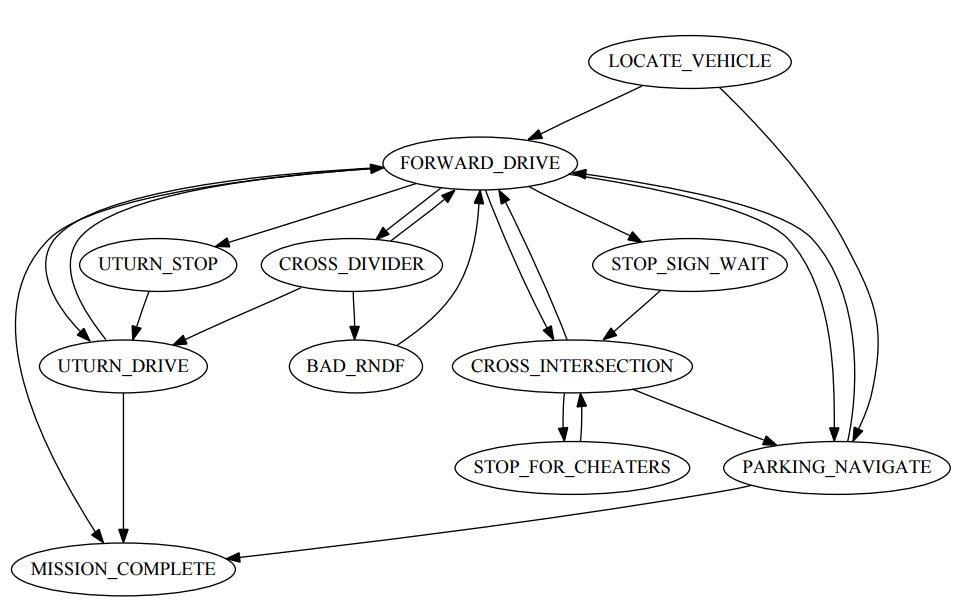
\includegraphics[width=10cm]{Junior.png}
\caption[Junior的状态转移图]{Junior的状态转移图\cite{Montemerlo2008Junior}}
\label{fig:junior}
\end{figure}

\begin{figure}[htbp]
\centering
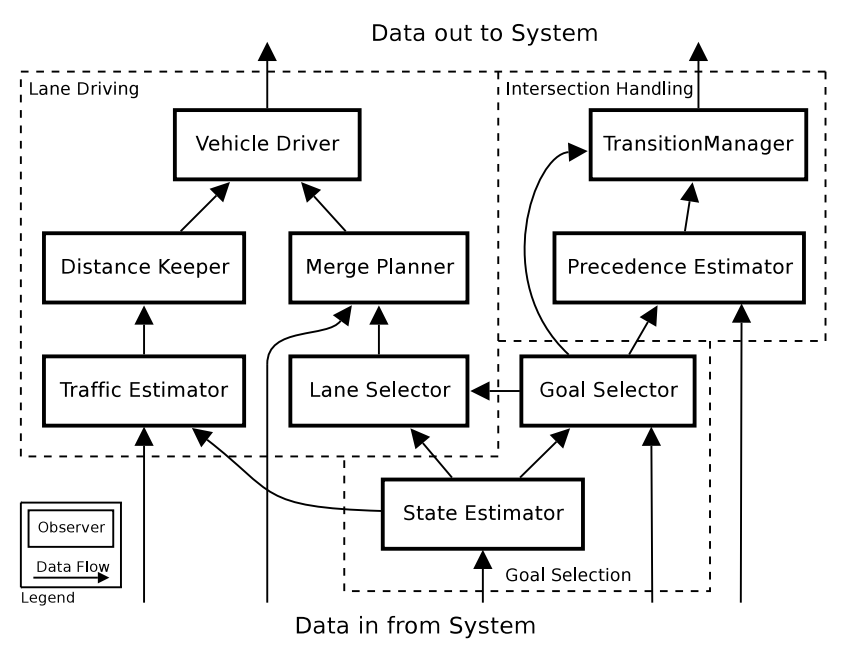
\includegraphics[width=10cm]{BOSS.png}
\caption[BOSS的行为决策流程]{BOSS的行为决策流程\cite{Baker2008Traffic}}
\label{fig:boss}
\end{figure}

这种状态机方法往往仅能在特定情况下正常工作,而现实中的交通场景变化多端,只依靠预先确定的状态和规则不能保证控制的安全性。

\item 规则学习方法。
如果无人车可以很好的模拟人的驾驶行为,可以直接解决行为决策的问题。因此,行为决策和驾驶行为预测是紧密相关的,行为决策的规则可以从实际驾驶行为数据中进行学习。使用贝叶斯算法可以完成这一点。例如,Kumar P.等人\cite{Kumar2013Learning}使用贝叶斯方法对驾驶员数据进行分析,预测车道汇合时的驾驶员意图。Lidstrom K. 等人\cite{Lidstrom2008Model}指出动态贝叶斯网络(Dynamic Bayesian Model, DBN)可以用来处理不确定的时空依赖性。决策树也可以用于规则的学习。例如Schubert R.\cite{Schubert2012Evaluating}利用决策树能融知 识表示与获取于一身的优点,将决策树用不同驾驶行为机制的研究,以实现 对驾驶员行为的模拟再现。人工神经网络具有高度非线性映射能力,在智能控制中有广泛应用。例如 Chong L.等人\cite{Chong2013A}提出了一种基于模糊规则的神经网络从车辆轨迹预测驾驶员的驾驶行为。

诸如此类的规则学习方法还有很多种。这类方法在经过线下学习之后可以在各种场景下快速决定驾驶行为,但由于实际驾驶环境还有很多不确定性,对环境的感知也可能存在不一致的情况,对行为的决策最好能够考虑这种不确定性。

\item 不确定性的建模。
考虑到其他车辆的行为是不确定的,行为决策系统经常使用概率模型,例如马尔科夫决策过程(Markov Decision Process, MDP)及其推广形式。\cite{Brechtel2011Probabilistic}即使用了MDP模型解决无人车的行为决策问题。另外一些工作将未观察到的驾驶场景和行人意图使用 partially-observable MDP (POMDB)建模,由此估计驾驶场景并进行行为决策。例如\inlinecite{Ulbrich2013Probabilistic}提出了如图\ref{fig:POMDB}所示的两步决策过程,减小了传感器噪声对车道变换中行为决策的影响。
\end{enumerate}

\begin{figure}[htbp]
\centering
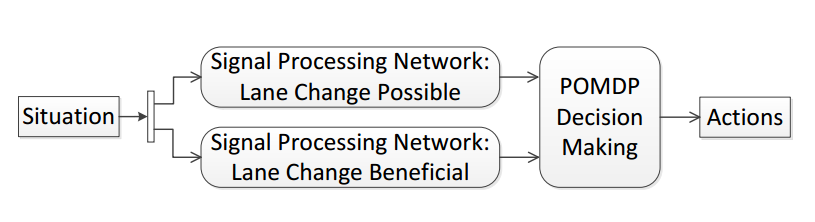
\includegraphics[width=13cm]{POMDB.png}
\caption[POMDB在车道转换中的决策过程]{POMDB在车道转换中的决策过程\cite{Ulbrich2013Probabilistic}}
\label{fig:POMDB}
\end{figure}

\item \textbf{轨迹规划算法综述}
\label{sec:trajectory}

轨迹规划问题又可以根据是否将时间当做自变量,分为路线(Path)规划和轨线(Trajectory)规划。其中路线规划获得的路线可表达为函数 $\sigma(\alpha): [0,1]\rightarrow \mathcal{X}$,其中$\mathcal{X}$为车辆的构形空间(Configuration Space,指规划范围内空间位置的集合)。对于轨线规划问题,获得的轨线可表达为函数 $\pi(t): [0, T]\rightarrow \mathcal{X}$,其中$T$为规划时限。

\begin{enumerate}[label=(\arabic*),wide=\parindent]
\item 路线规划。 路线规划问题就是从初始构形开始,求得能够到达目标区域的满足全局和局部约束的路线。根据路线规划的目标,路线规划又可分为\textbf{可行路线规划}和\textbf{最优路线规划}。令$\mathcal{X}$表示车辆的构形空间,$\Sigma(\mathcal{X})$表示所有$[0,1]\rightarrow \mathcal{X}$的连续函数的集合,$\mathbf{x}_{\mathrm{init}}\in \mathcal{X}$表示初始构形,$X_{\mathrm{goal}}\subseteq \mathcal{X}$表示目标区域。车辆可达区域构成自由构形空间$\mathcal{X}_{\mathrm{free}}$。此外,车辆路线还需要满足一系列阶次的约束,表示为$D(\mathbf{x},\mathbf{x}',\mathbf{x}'', \dots)$,对于最优路线规划的描述如下:

\begin{definition}[最优路线规划]
\label{def:path}
给定五元组$(\mathcal{X}_{\mathrm{free}}, \mathbf{x}_{\mathrm{init}}, X_{\mathrm{goal}}, D, J)$ 找出$\sigma^*=$
\begin{equation}
\begin{aligned}
\underset{\sigma\in \Sigma(\mathcal{X})}{\arg\min}\quad & J(\sigma) & \\
\mathrm{subj. to} \quad & \sigma(0)=\mathbf{x}_{\mathrm{init}} \quad \mathrm{and} \quad \sigma(1)\in X_{goal} & \\
\quad & \sigma(\alpha)\in \mathcal{X}_{\mathrm{free}} & \quad \forall \alpha\in [0,1]\\
& D(\sigma(\alpha),\sigma'(\alpha),\sigma''(\alpha), \dots) & \forall \alpha\in [0,1]
\end{aligned}
\end{equation}
\end{definition}

最优路线规划已经被证明是 PSPACE难的问题\cite{Reif1979Complexity}。如果假设 $\mathrm{P}\neq \mathrm{NP}$,则不存在多项式复杂度的算法,能够在任何情况下解最优路线规划问题。对于求解可行路线规划,在1979年,Reif\cite{Reif1979Complexity}研究了完整车辆(holonomic vehicle,不存在非完整性约束)在二维、三维环境中寻找可行路线的问题,提出了一种多项式复杂度的算法。Canny\cite{Canny1988The}证明了用多边形表示自由构形空间,不存在高阶约束时,可行路线规划问题是PSPACE完全的。

对于最优路线规划,常见的目标是求得最短的无障碍路径。在该目标下,对于完整车辆,在二维多边形障碍的构形空间中存在多项式时间的算法\cite{Storer1994Shortest,Lozano1979An}。更准确地讲,存在复杂度为$O(n^2)$的算法,其中$n$为空间中车辆数目。该方法是基于可见性图的。

\item 轨线规划。 与路线规划类似,最优轨线规划问题的定义如下:

\begin{definition}[最优轨线规划]
\label{def:trajectory}
给定六元组$(\mathcal{X}_{\mathrm{free}}, \mathbf{x}_{\mathrm{init}}, X_{\mathrm{goal}}, D, J, T)$ 找出$\pi^*=$
\begin{equation}
\begin{aligned}
\underset{\pi\in \Sigma(\mathcal{X})}{\arg\min}\quad & J(\pi) & \\
\mathrm{subj. to} \quad & \pi(0)=\mathbf{x}_{\mathrm{init}} \quad \mathrm{and} \quad \pi(1)\in X_{goal} & \\
\quad & \pi(t)\in \mathcal{X}_{\mathrm{free}} & \quad \forall t\in [0,1]\\
& D(\pi(t),\pi'(t),\pi''(t), \dots) & \forall t\in [0,1]
\end{aligned}
\end{equation}
\end{definition}

由于轨线规划是路线规划的推广,最优轨线规划仍是PSPACE难的。Canny和Reif\cite{Canny1987New}证明了对于有速度约束的完整车辆,在二维多边形障碍的共性空间中找到最短无障碍轨线是NP难的。注意到同样环境下的路线规划问题是存在$O(n^2)$算法的。该环境是无人车控制的典型环境。由于不存在有效的算法能够求得精确解,通常采用数值解法。
\end{enumerate}

\item \textbf{轨迹规划的数值解法 }

常用的数值解法可以分为以下三大类:

\begin{enumerate}[label=(\arabic*),wide=\parindent]
% \begin{enumerate}
\item 变分法(Variational methods)提取一组参数,将最优路线或轨线的求解问题转化为在该参数空间的搜索问题,优化的函数往往是非线性的。这种方法收敛较快,但不能保证收敛到全局最优。\inlinecite{Ziegler2014Making}将优化问题转化为数值积分问题,并使用欧拉法优化。\inlinecite{Darby2011An}进一步用一组基函数表示插值函数,获得了更快的收敛速度。对于变分法更详细的综述,参见\inlinecite{Betts1998Survey}。

\item 图搜索算法(Graph-search methods)将构形空间离散化为有限的顶点而生成图,图的边表示顶点之间的转移关系。最优路线或轨线的求解可转化为在图中求最小费用路径的问题。图\ref{fig:graph}为一个人工标定的车道图示例。生成该图除了人工标定,也可以从地理图片生成\cite{Backer2007Finding,Wang1996Approximation},或从观测到的构形空间采样生成\cite{Lavalle1999Rapidly,Glassman2010A}。获得了道路结构图之后,可以使用Dijkstra算法\cite{Dijkstra1959A}或$A^*$启发式搜索\cite{Hart2010A}。图搜索方法虽然能够获得全局最优,但得到的最优路径只是在由离散的构形空间点上的最优路径,而在整个构形空间上可能是次优的。有时这种方法甚至无法得到可行路径。

\item 递增搜索算法(Incremental search methods)增量地寻找可行路径。如果存在可行路径,该方法在计算时间足够的情况下总能找到可行路径。若要求寻找最优路径,该方法可以进一步给出一列渐优的路径,逐渐收敛到最优路径。\inlinecite{David1997Path}提出了一种基于可扩展空间树(expansive spaces tree, EST)的方法,每次随机从当前所有节点中选择一个扩展节点,在以该节点为中心的圆形区域采样得到扩展的节点。La Valle\cite{Lavalle1999Rapidly}提出了一种快速探索的随机扩展树(Rapid-exploring Random Tree, RRT),能够快速在高阶非完整系统中找到可行路径。
\end{enumerate}

\begin{figure}[htbp]
\centering
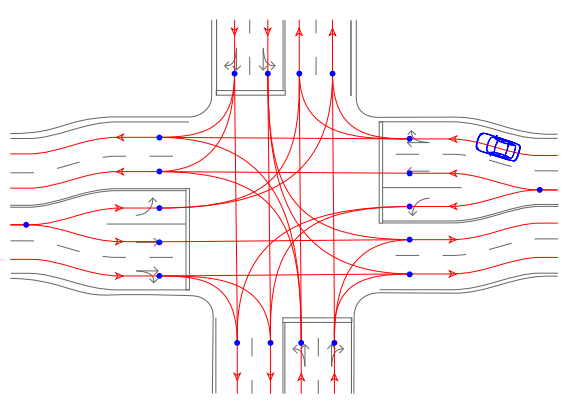
\includegraphics[width=8cm]{graph.png}
\caption{典型道路拓扑图}
\label{fig:graph}
\end{figure}

\item \textbf{多智能车决策问题}
\label{sec:multi}

上述无人车研究均只涉及了单车的控制问题。如果在多车群决策系统中进行优化,即使使用简单的车辆模型,往往也能达到和单车分别决策相同,甚至更好的效果\cite{Cao2012An}。由于车路协同平台的发展,对于多智能车的协同控制,即群决策应用的需求也越来越大。多车的协同控制是具有广阔前景的研究领域。

多智能车协作问题是多智能体系统(Multi-Agent System, MAS)的具体应用。其控制方法可分为中心化方法和分布式方法两种。前者需要有强大的计算中心支持,一个中心需要处理大量车辆的决策问题。本质上,该方法是单车控制策略的拓展,仍可使用单车控制中的一系列方法进行类似的处理。而后者则将计算任务分配到每个车辆,省去了计算中心,但会使整个系统的结构和组织更为复杂。

由于本课题研究车道汇合处的决策问题,下面将针对车道汇合场景进行多智能车决策问题的综述。基于车路协同平台,车辆之间的通信方式、控制方式都和传统的单车决策、信号灯控制有很大不同。在该环境下,对车道汇合问题的研究主要分为三方面:

\begin{enumerate}[label=(\arabic*),wide=\parindent]
% \begin{enumerate}
\item 研究新的通信方式下如何提高交通通行效率和安全性;
\item 研究通信本身的可靠性和对车道汇合问题的影响;
\item 实验仿真车或其他机器人在汇合场景的表现。
\end{enumerate}

下文将对这三方面分别展开综述。

% \item \textbf{研究问题}
% 计划群决策的三个层次:
% 信息方面的决策
% 基于决策的决策
% 行为预测,决策协作?

\begin{enumerate}[label=(\arabic*),wide=\parindent]
\item 安全性和效率问题。
根据前文单车轨迹规划的背景知识,车辆轨迹规划可以通过设计不同的目标函数而达到不同的优化效果。同样的,多车的轨迹规划问题也可以通过设计多车协作的整体目标来权衡安全性和效率。在较早的车道汇合研究中,\inlinecite{Kanaris2001Strategies}将目标选取为优化交通流的分布,\inlinecite{Raravi2007Merge}则着重优化车辆通过交叉路口的总时间,但忽略了车辆汇合的顺序问题,这可能造成不公平。\inlinecite{Baselt2014Merging}则将公平性也作为一种目标,提出了一种名为“自由流”(free-flow)的公平性度量。为了考察多车协同的有效性,\inlinecite{Xu2002Effects}研究了存在与不存在车间通信的情况下,汇合点上游车队长度的问题。\inlinecite{Xu2003Simulation}考察了协同自主巡航系统(cooperative autonomous cruise control, C-ACC)和没有协同控制的自主巡航系统(autonomous cruise control, ACC)在汇合处对整体通行目标的影响。\inlinecite{Wang2009Robust}总结了车辆在交汇口的标准问题、决策方法和通信算法。\cite{Gradinescu2007Adaptive}使用传统交通信号灯控制方案研究了存在车车通信时十字路口的控制问题。

\item 通信可靠性问题。
\cite{Abbas2013Radio}讨论了车道汇合和交叉口场景中天线辐射模式对视野长度的影响。\inlinecite{Uno1999A}提出了一种车道汇合处无人车的控制算法,并研究了通信时延对算法的影响。

\item 仿真实验。
部分研究者从实验角度研究车辆在车道汇合场景的行为。如\inlinecite{Sakaguchi1999Inter,Kolodko2003Cooperative}等工作很早(1999, 2003年)就开始研究存在车间通信的情况下,车辆在车道汇合、十字路口等场景的控制问题。而时间较近的一个实验\cite{Milanes2011Automated}也研究了类似的场景,展示了车车协同在路口汇合场景中的可行性。该实验是AUTOPIA\cite{Milan2011AUTOPIA}项目的一部分。
\end{enumerate}

\subsection{总结}
\label{ssec:intro:summary}
从以上文献综述以及智能交通领域,尤其是多智能车协同控制领域近年的发展来看,可以得出以下结论:

\begin{enumerate}[label=(\arabic*),wide=\parindent]
% \begin{enumerate}
\item 行为决策问题还未解决。对于无人车控制的四个层次,整体路线规划已经有相当快速的算法,在轨迹追踪和反馈控制领域也有较为成熟的技术,但无人车行为决策的界限还很模糊,算法还不能适应各种场景。而这也是智能交通当今研究的重点领域之一。
\item 多智能车决策与实际联系较少。虽然多智能车的算法研究很早就开始了,并且在机器人编队领域有许多方法可以借鉴,但由于车辆的控制与基础设施密切相关,在没有统一通信标准时,许多场景只能靠假设,或进行纯理论的研究。仿真实验虽然在上世纪就已经开始,但实际道路中车辆通信的基础设施还不够完善,以至于十几年时间里,仿真内容仍然十分类似。当今车美国、欧洲纷纷提出了一些车路协同、多车协作的通信标准\cite{Chen2014Cooperative}。在这样的背景下,多车的决策控制问题又迎来了新的机遇与挑战。
\item 混合通行系统的协同控制问题研究很少。由于无人车技术的进步,未来很长一段时间的实际交通环境将由无人车和有人驾驶车辆共同参与。之前的研究要么着眼于驾驶员行为预测,要么研究多个完全可控车辆的车队等问题,在混合通行环境中的协同控制,或者混合通行环境对于智能车协同控制的影响还没有研究。
\end{enumerate}

\end{enumerate}

\section{研究内容}
基于以上的研究现状调研,并结合自动化系实际,本课题拟采用自动控制理论中所学的最优控制方法对车道交汇路口进行建模和分析,使用变分法对模型进行求解,对于无法获得解析解的情况,使用数值分析和运筹学中所学的方法求得数值解。具体来说,研究内容有以下几点:
\begin{enumerate}[label=(\arabic*),wide=\parindent]
% \begin{enumerate}
\item 对于车道交汇口场景的建模,最重要的问题是如何选取目标函数。本课题尝试最小化通行时间和系统总能量的方法,并尝试了优先时间下界的优化和将时间、能量因素融合的方法;
\item 交汇口的车辆通行顺序是影响控制目标的一个重要因素。本课题将分析多种通行顺序决策方式。除了传统的先进先出策略,本课题将提出一种基于最优通行时间的排序方法,并与先进先出的方案进行比较分析;
\item 为了对课题中提出的算法进行仿真,而避免专业仿真软件的一些冗余设定,本文作者基于{\ttfamily Python}语言自主开发了一套仿真程序框架和一个简单的网页应用。
\end{enumerate}

本课题的研究意义在于:
\begin{enumerate}[label=(\arabic*),wide=\parindent]
% \begin{enumerate}[label=(\arabic*),itemindent=\dimexpr\labelwidth+\labelsep\relax,leftmargin=0pt]
% \begin{enumerate}
\item 智能车是富有前景的未来交通工具,本课题控制的车辆是完全可控的智能车,该场景既是混合通行场景的基础,是智能车控制从理论走向实际的第一步;
\item 车路协同平台为多智能车的群决策提供了支持,群决策相比于个体决策能达到更高的通行效率,但对于利用群决策提高通行效率的理论研究还比较少,本文将填补这一空白;
\item 智能交通研究中的各种场景都可以作为多智能车群决策问题的背景,本课题所研究的交汇口场景是复杂场景研究的基础,且本课题提出的算法框架可以比较容易的推广到交叉口场景。
\end{enumerate}

\section{论文组织}
后文的组织结构如下:第\ref{cha:algorithm}章建立了车道汇合群决策系统的模型和约束条件,提出了目标函数,并运用安全性约束确定了通行时间的下限;第\ref{cha:solve}章运用变分法,在不同的约束条件下对模型进行求解,并描述了基于最优通行时间的排序原理;第\ref{cha:sim}在多种情况下对算法进行了仿真;第\ref{cha:sum}对本文进行了总结,并提出了未来的研究方向。